\documentclass[]{article}
\usepackage[T1]{fontenc}
\usepackage{lmodern}
\usepackage{amssymb,amsmath}
\usepackage{ifxetex,ifluatex}
\usepackage{fixltx2e} % provides \textsubscript
\usepackage{graphicx}
% Redefine \includegraphics so that, unless explicit options are
% given, the image width will not exceed the width of the page.
% Images get their normal width if they fit onto the page, but
% are scaled down if they would overflow the margins.
\makeatletter
\def\ScaleIfNeeded{%
  \ifdim\Gin@nat@width>\linewidth
    \linewidth
  \else
    \Gin@nat@width
  \fi
}
\makeatother
\let\Oldincludegraphics\includegraphics
{%
 \catcode`\@=11\relax%
 \gdef\includegraphics{\@ifnextchar[{\Oldincludegraphics}{\Oldincludegraphics[width=\ScaleIfNeeded]}}%
}%
% use upquote if available, for straight quotes in verbatim environments
\IfFileExists{upquote.sty}{\usepackage{upquote}}{}
\ifnum 0\ifxetex 1\fi\ifluatex 1\fi=0 % if pdftex
  \usepackage[utf8]{inputenc}
\else % if luatex or xelatex
  \ifxetex
    \usepackage{mathspec}
    \usepackage{xltxtra,xunicode}
  \else
    \usepackage{fontspec}
  \fi
  \defaultfontfeatures{Mapping=tex-text,Scale=MatchLowercase}
  \newcommand{\euro}{€}
\fi
% use microtype if available
\IfFileExists{microtype.sty}{\usepackage{microtype}}{}
\usepackage{longtable}
\ifxetex
  \usepackage[setpagesize=false, % page size defined by xetex
              unicode=false, % unicode breaks when used with xetex
              xetex]{hyperref}
\else
  \usepackage[unicode=true]{hyperref}
\fi
\hypersetup{breaklinks=true,
            bookmarks=true,
            pdfauthor={},
            pdftitle={Type Checking},
            colorlinks=true,
            citecolor=blue,
            urlcolor=blue,
            linkcolor=magenta,
            pdfborder={0 0 0}}
\urlstyle{same}  % don't use monospace font for urls
\setlength{\parindent}{0pt}
\setlength{\parskip}{6pt plus 2pt minus 1pt}
\setlength{\emergencystretch}{3em}  % prevent overfull lines
\setcounter{secnumdepth}{5}

\title{The Cool Reference Manual\footnote{Cool and the Cool Reference Manual Copyright ©1995-2006 by Alex Aiken. All rights reserved. This version of the Cool Reference Manual has been modified by Wes Weimer. All of the good things herein should be credited to Alex Aiken. All mistakes should be attributed to Wes Weimer.}}

\begin{document}
\maketitle
\tableofcontents

\section{Attributes}

An attribute definition has the form

\begin{verbatim}
<id> : <type> [ <- <expr> ];
\end{verbatim}

The expression is optional initialization that is executed when a new
object is created. The static type of the expression must conform to the
declared type of the attribute. If no initialization is supplied, then
the default initialization is used (see below).

When a new object of a class is created, all of the inherited and local
attributes must be initialized. Inherited attributes are initialized
first in inheritance order beginning with the attributes of the greatest
ancestor class. Within a given class, attributes are initialized in the
order they appear in the source text.

Attributes are local to the class in which they are defined or
inherited. Inherited attributes cannot be redefined.


\subsection{Void}

All variables in Cool are initialized to contain values of the
appropriate type. The special value \texttt{void} is a member of all
types and is used as the default initialization for variables where no
initialization is supplied by the user. (\texttt{void} is used where one
would use \texttt{NULL} in C or \texttt{null} in Java; Cool does not
have anything equivalent to C's or Java's \texttt{void} type.) Note that
there is no name for \texttt{void} in Cool; the only way to create a
\texttt{void} value is to declare a variable of some class other than
\texttt{Int}, \texttt{String}, or \texttt{Bool} and allow the default
initialization to occur, or to store the result of a \texttt{while}
loop.

There is a special form \texttt{isvoid expr} that tests whether a value
is \texttt{void} (see Section~\href{node24.html\#sec-isvoid}{7.11}). In
addition, \texttt{void} values may be tested for equality. A
\texttt{void} value may be passed as an argument, assigned to a
variable, or otherwise used in any context where any value is
legitimate, except that a dispatch to or case on \texttt{void} generates
a runtime error.

Variables of the basic classes \texttt{Int}, \texttt{Bool}, and
\texttt{String} are initialized specially; see
Section~\href{node26.html\#sec-basic}{8}.

\section{Methods}

A method definition has the form

\begin{verbatim}
<id>(<id> : <type>,...,<id> : <type>): <type> { <expr> };
\end{verbatim}

There may be zero or more formal parameters. The identifiers used in the
formal parameter list must be distinct. The type of the method body must
conform to the declared return type. When a method is invoked, the
formal parameters are bound to the actual arguments and the expression
is evaluated; the resulting value is the meaning of the method
invocation. A formal parameter hides any definition of an attribute of
the same name.

To ensure type safety, there are restrictions on the redefinition of
inherited methods. The rule is simple: If a class \texttt{C} inherits a
method \texttt{f} from an ancestor class \texttt{P}, then \texttt{C} may
override the inherited definition of \texttt{f} provided the number of
arguments, the types of the formal parameters, and the return type are
exactly the same in both definitions.

To see why some restriction is necessary on the redefinition of
inherited methods, consider the following example:

\begin{verbatim}
class P {
   f(): Int { 1 };
};

class C inherits P {
   f(): String { "1" };
};
\end{verbatim}

Let \texttt{p} be an object with dynamic type \texttt{P}. Then

\begin{verbatim}
p.f() + 1
\end{verbatim}

is a well-formed expression with value 2. However, we cannot substitute
a value of type \texttt{C} for \texttt{p}, as it would result in adding
a string to a number. Thus, if methods can be redefined arbitrarily,
then subclasses may not simply extend the behavior of their parents, and
much of the usefulness of inheritance, as well as type safety, is lost.


\section{Expressions}

Expressions are the largest syntactic category in Cool. \\


\subsection{Constants}

The simplest expressions are constants. The boolean constants are
\texttt{true} and \texttt{false}. Integer constants are unsigned strings
of digits such as \texttt{0}, \texttt{123}, and \texttt{007}. String
constants are sequences of characters enclosed in double quotes, such as
\texttt{"This is a string."} String constants may be at most 1024
characters long. There are other restrictions on strings; see
Section~\href{node33.html\#lex-struct}{10}.

The constants belong to the basic classes \texttt{Bool}, \texttt{Int},
and \texttt{String}. The value of a constant is an object of the
appropriate basic class.

\subsection{Identifiers}

The names of local variables, formal parameters of methods,
\texttt{self}, and class attributes are all expressions. The identifier
\texttt{self} may be referenced, but it is an error to assign to
\texttt{self} or to bind \texttt{self} in a \texttt{let}, a
\texttt{case}, or as a formal parameter. It is also illegal to have
attributes named \texttt{self}.

Local variables and formal parameters have lexical scope. Attributes are
visible throughout a class in which they are declared or inherited,
although they may be hidden by local declarations within expressions.
The binding of an identifier reference is the innermost scope that
contains a declaration for that identifier, or to the attribute of the
same name if there is no other declaration. The exception to this rule
is the identifier \texttt{self}, which is implicitly bound in every
class.

\subsection{Assignment}

An assignment has the form

\begin{verbatim}
<id> <- <expr>
\end{verbatim}

The static type of the expression must conform to the declared type of
the identifier. The value is the value of the expression. The static
type of an assignment is the static type of
\texttt{\textless{}expr\textgreater{}}.

\subsection{Dispatch}

There are three forms of dispatch (i.e. method call) in Cool. The three
forms differ only in how the called method is selected. The most
commonly used form of dispatch is

\begin{verbatim}
<expr>.<id>(<expr>,...,<expr>)
\end{verbatim}

Consider the dispatch $\tt e_0.f(e_1,\ldots,e_n)$. To evaluate this
expression, the arguments are evaluated in left-to-right order, from
$\tt e_1$ to $\tt e_n$. Next, $\tt e_0$ is evaluated and its class
\texttt{C} noted (if $\tt e_0$ is \texttt{void} a runtime error is
generated). Finally, the method \texttt{f} in class \texttt{C} is
invoked, with the value of $\tt e_0$ bound to \texttt{self} in the body
of \texttt{f} and the actual arguments bound to the formals as usual.
The value of the expression is the value returned by the method
invocation.

Type checking a dispatch involves several steps. Assume $\tt e_0$ has
static type \texttt{A}. (Recall that this type is not necessarily the
same as the type \texttt{C} above. \texttt{A} is the type inferred by
the type checker; \texttt{C} is the class of the object computed at
runtime, which is potentially any subclass of \texttt{A}.) Class
\texttt{A} must have a method \texttt{f}, the dispatch and the
definition of \texttt{f} must have the same number of arguments, and the
static type of the $i$th actual parameter must conform to the declared
type of the $i$th formal parameter.

If \texttt{f} has return type \texttt{B} and \texttt{B} is a class name,
then the static type of the dispatch is \texttt{B}. Otherwise, if
\texttt{f} has return type \texttt{SELF\_TYPE}, then the static type of
the dispatch is \texttt{A}. To see why this is sound, note that the
\texttt{self} parameter of the method \texttt{f} conforms to type
\texttt{A}. Therefore, because \texttt{f} returns \texttt{SELF\_TYPE},
we can infer that the result must also conform to \texttt{A}. Inferring
accurate static types for dispatch expressions is what justifies
including \texttt{SELF\_TYPE} in the Cool type system.

The other forms of dispatch are:

\begin{verbatim}
<id>(<expr>,...,<expr>)
<expr>@<type>.id(<expr>,...,<expr>)
\end{verbatim}

The first form is shorthand for
\texttt{self.\textless{}id\textgreater{}(\textless{}expr\textgreater{},...,\textless{}expr\textgreater{})}.

The second form provides a way of accessing methods of parent classes
that have been hidden by redefinitions in child classes. Instead of
using the class of the leftmost expression to determine the method, the
method of the class explicitly specified is used. For example,
\texttt{e@B.f()} invokes the method \texttt{f} in class \texttt{B} on
the object that is the value of \texttt{e}. For this form of dispatch,
the static type to the left of ``@'`must conform to the type specified
to the right of ``@''.

\subsection{Conditionals}

A conditional has the form

\begin{verbatim}
if <expr> then <expr> else <expr> fi
\end{verbatim}

The semantics of conditionals is standard. The predicate is evaluated
first. If the predicate is \texttt{true}, then the \texttt{then} branch
is evaluated. If the predicate is \texttt{false}, then the \texttt{else}
branch is evaluated. The value of the conditional is the value of the
evaluated branch.

The predicate must have static type \texttt{Bool}. The branches may have
any static types. To specify the static type of the conditional, we
define an operation $\sqcup$ (pronounced ``join'') on types as follows.
Let \texttt{A,B,D} be any types other than \texttt{SELF\_TYPE}. The
\emph{least type} of a set of types means the least element with respect
to the conformance relation $\leq$. \\

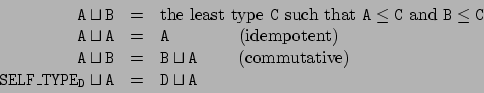
\includegraphics{img23.png}

Let \texttt{T} and \texttt{F} be the static types of the branches of the
conditional. Then the static type of the conditional is
$\tt T \sqcup F$. (think: Walk towards \texttt{Object} from each of
\texttt{T} and \texttt{F} until the paths meet.)

\subsection{Loops}

A loop has the form

\begin{verbatim}
while <expr> loop <expr> pool
\end{verbatim}

The predicate is evaluated before each iteration of the loop. If the
predicate is \texttt{false}, the loop terminates and \texttt{void} is
returned. If the predicate is \texttt{true}, the body of the loop is
evaluated and the process repeats.

The predicate must have static type \texttt{Bool}. The body may have any
static type. The static type of a loop expression is \texttt{Object}.

\subsection{Blocks}

A block has the form

\begin{verbatim}
{ <expr>; ... <expr>; }
\end{verbatim}

The expressions are evaluated in left-to-right order. Every block has at
least one expression; the value of a block is the value of the last
expression. The expressions of a block may have any static types. The
static type of a block is the static type of the last expression.

An occasional source of confusion in Cool is the use of semi-colons
(``\texttt{;}''). Semi-colons are used as terminators in lists of
expressions (e.g., the block syntax above) and not as expression
separators. Semi-colons also terminate other Cool constructs, see
Section~\href{node39.html\#sec-gram}{11} for details.

\subsection{Let}

A let expression has the form

\begin{verbatim}
let <id1> : <type1> [ <- <expr1> ], ..., <idn> : <typen> [ <- <exprn> ] in <expr>
\end{verbatim}

The optional expressions are \emph{initialization}; the other expression
is the \emph{body}. A \texttt{let} is evaluated as follows. First
\texttt{\textless{}expr1\textgreater{}} is evaluated and the result
bound to \texttt{\textless{}id1\textgreater{}}. Then
\texttt{\textless{}expr2\textgreater{}} is evaluated and the result
bound to \texttt{\textless{}id2\textgreater{}}, and so on, until all of
the variables in the \texttt{let} are initialized. (If the
initialization of \texttt{\textless{}idk\textgreater{}} is omitted, the
default initialization of type \texttt{\textless{}typek\textgreater{}}
is used.) Next the body of the \texttt{let} is evaluated. The value of
the \texttt{let} is the value of the body.

The \texttt{let} identifiers
\texttt{\textless{}id1\textgreater{},...,\textless{}idn\textgreater{}}
are visible in the body of the \texttt{let}. Furthermore, identifiers
\texttt{\textless{}id1\textgreater{},...,\textless{}idk\textgreater{}}
are visible in the initialization of
\texttt{\textless{}idm\textgreater{}} for any
\texttt{m \textgreater{} k}.

If an identifier is defined multiple times in a \texttt{let}, later
bindings hide earlier ones. Identifiers introduced by \texttt{let} also
hide any definitions for the same names in containing scopes. Every
\texttt{let} expression must introduce at least one identifier.

The type of an initialization expression must conform to the declared
type of the identifier. The type of \texttt{let} is the type of the
body.

The \texttt{\textless{}expr\textgreater{}} of a \texttt{let} extends as
far (encompasses as many tokens) as the grammar allows.

A case expression has the form

\begin{verbatim}
case <expr0> of 
    <id1> : <type1> => <expr1>; 
    . . .
    <idn> : <typen> => <exprn>; 
esac
\end{verbatim}

Case expressions provide runtime type tests on objects. First,
\texttt{expr0} is evaluated and its dynamic type \texttt{C} noted (if
\texttt{expr0} evaluates to \texttt{void} a run-time error is produced).
Next, from among the branches the branch with the least type
\texttt{\textless{}typek\textgreater{}} such that
\texttt{C  \textless{}typek\textgreater{}} is selected. The identifier
\texttt{\textless{}idk\textgreater{}} is bound to the value of
\texttt{\textless{}expr0\textgreater{}} and the expression
\texttt{\textless{}exprk\textgreater{}} is evaluated. The result of the
\texttt{case} is the value of \texttt{\textless{}exprk\textgreater{}}.
If no branch can be selected for evaluation, a run-time error is
generated. Every \texttt{case} expression must have at least one branch.

For each branch, let $\tt T_i$ be the static type of
\texttt{\textless{}expri\textgreater{}}. The static type of a
\texttt{case} expression is $\tt\bigsqcup_{1 \leq i \leq
n} T_i$. The identifier \texttt{id} introduced by a branch of a
\texttt{case} hides any variable or attribute definition for \texttt{id}
visible in the containing scope.

The \texttt{case} expression has no special construct for a
``default'`or ``otherwise'' branch. The same affect is achieved by
including a branch

\begin{verbatim}
   x : Object => ...
\end{verbatim}

because every type is 
\includegraphics{img22.png} to \texttt{Object}.

The \texttt{case} expression provides programmers a way to insert
explicit runtime type checks in situations where static types inferred
by the type checker are too conservative. A typical situation is that a
programmer writes an expression 
\includegraphics{img27.png} and type
checking infers that 
\includegraphics{img27.png} has static type

\includegraphics{img3.png}. However, the programmer may know that, in
fact, the dynamic type of 
\includegraphics{img27.png} is always

\includegraphics{img28.png} for some 
\includegraphics{img1.png}. This
information can be captured using a case expression:

\begin{verbatim}
case e of x : C => ...
\end{verbatim}

In the branch the variable 
\includegraphics{img29.png} is bound to the
value of 
\includegraphics{img27.png} but has the more specific static
type 
\includegraphics{img28.png}.

\subsection{New}

A \texttt{new} expression has the form

\begin{verbatim}
new <type>
\end{verbatim}

The value is a fresh object of the appropriate class. If the type is
\texttt{SELF\_TYPE}, then the value is a fresh object of the class of
\texttt{self} in the current scope. The static type is
\texttt{\textless{}type\textgreater{}}.

\subsection{Isvoid}

The expression

\begin{verbatim}
isvoid expr
\end{verbatim}

evaluates to \texttt{true} if \texttt{expr} is \texttt{void} and
evaluates to \texttt{false} if \texttt{expr} is not \texttt{void}.

\subsection{Arithmetic and Comparison Operations}

\paragraph{Binary Arithmetic}

Cool has four binary arithmetic operations: \texttt{+, -, *, /}. The
syntax is

\begin{verbatim}
expr1 <op> expr2
\end{verbatim}

To evaluate such an expression first \texttt{expr1} is evaluated and
then \texttt{expr2}. The result of the operation is the result of the
expression.

The static types of the two sub-expressions must be \texttt{Int}. The
static type of the entire arithmetic expression is also \texttt{Int}.
Cool has only integer division.

\paragraph{Binary Relations}

Cool has three comparison operations:
\texttt{\textless{}, \textless{}=, =}. These comparisons may be applied
to subexpressions of any types, subject to the following rules:

\begin{itemize}
\itemsep1pt\parskip0pt\parsep0pt
\item
  \texttt{expr1} is an \texttt{Int} if and only if \texttt{expr2} is an
  \texttt{Int}
\item
  \texttt{expr1} is a \texttt{String} if and only if \texttt{expr2} is a
  \texttt{String}
\item
  \texttt{expr1} is a \texttt{Bool} if and only if \texttt{expr2} is a
  \texttt{Bool}
\item
  Otherwise, \texttt{expr1} may be of any type (including
  \texttt{SELF\_TYPE}) and \texttt{expr2} may be of any (possibly
  different) type (including \texttt{SELF\_TYPE}).
\end{itemize}

In all cases, the result of the comparison is a \texttt{Bool}. See
\href{node43.html}{the type checking rules} for more information.

In principle, there is nothing wrong with permitting equality tests
between, for example, \texttt{Bool} and \texttt{Int}. However, such a
test must always be false and almost certainly indicates some sort of
programming error. The Cool type checking rules catch such errors at
compile-time instead of waiting until runtime.

On non-basic objects, equality is decided via pointer equality (i.e.,
whether the memory addresses of the objects are the same). Equality is
defined for \texttt{void}: two \texttt{void} values are equal and a
\texttt{void} value is never equal to a non-\texttt{void} value. See
\href{node48.html}{the operational semantics rules} for more
informaiton.

\paragraph{Unary Expressions}

Finally, there is one unary arithmetic and one unary logical operator.

\begin{itemize}
\itemsep1pt\parskip0pt\parsep0pt
\item
  The expression
  \texttt{\textasciitilde{} \textless{}expr\textgreater{}} is the
  integer complement of \texttt{\textless{}expr\textgreater{}}. The
  subexpression \texttt{\textless{}expr\textgreater{}} must have static
  type \texttt{Int} and the entire expression has static type
  \texttt{Int}.
\item
  The expression \texttt{not \textless{}expr\textgreater{}} is the
  boolean complement of \texttt{\textless{}expr\textgreater{}}. The
  subexpression \texttt{\textless{}expr\textgreater{}} must have static
  type \texttt{Bool} and the entire expression has static type
  \texttt{Bool}.
\end{itemize}

\section{Basic Classes}

\subsection{Object}

The \texttt{Object} class is the root of the inheritance graph. Even the
other basic classes (e.g., IO and Int) inherit from Object (and thus
inherit the three methods listed below). It is an error to redefine
\texttt{Object}. Methods with the following declarations are defined:

\begin{verbatim}
abort() : Object
type_name() : String
copy() : SELF_TYPE
\end{verbatim}

The method \texttt{abort} flushes all output and then halts program
execution with the error message \texttt{"abort\textbackslash{}n"}.

The method \texttt{type\_name} returns a string with the name of the
(run-time, dynamic) class of the object. The method \texttt{copy}
produces a \emph{shallow} copy of the
object.\href{footnode.html\#foot715}{\textsuperscript{4}}


\subsection{IO}

The \texttt{IO} class provides the following methods for performing
simple input and output operations:

\begin{verbatim}
out_string(x : String) : SELF_TYPE
out_int(x : Int) : SELF_TYPE
in_string() : String
in_int() : Int
\end{verbatim}

The methods \texttt{out\_string} and \texttt{out\_int} print their
argument, flush the standard output, and return their \texttt{self}
parameter.

The interpreter or compiler changes every \texttt{\textbackslash{}t} to
a tab and every \texttt{\textbackslash{}n} to a newline in the argument
\texttt{x} to \texttt{out\_string} before emitting the resulting string.
Note that this is different from normal escape sequence handling, where
\texttt{\textbackslash{}n} would be a single character stored in the
string. In Cool, it is two characters, but \texttt{out\_string} prints a
newline instead of \texttt{\textbackslash{}n}.

The method \texttt{in\_string} reads a string from the standard input,
up to but not including a newline character or the end of file. The
newline character is consumed but is not made part of the returned
string. If an error occurs then \texttt{in\_string} returns \texttt{""},
the string of length 0. Note that while literal lexical string constants
are limited to size 1024, strings generated by \texttt{in\_string} (or
\texttt{String.concat}, etc.) can be of arbitrary size. There is no
special processing of the two-character sequences
\texttt{\textbackslash{}t} or \texttt{\textbackslash{}n} (or, indeed
\texttt{\textbackslash{}anything}) during \texttt{in\_string}. Errors
include:

\begin{itemize}
\itemsep1pt\parskip0pt\parsep0pt
\item
  no input found before end of file
\item
  string read in contains NUL, the character with ASCII value 0 (in
  which case the entire string is rejected, even if there are valid
  characters around the NUL)
\end{itemize}

The method \texttt{in\_int} reads a single possibly-signed integer,
which may be preceded by whitespace. Any characters following the
integer, up to and including the next newline, are discarded by
\texttt{in\_int}. If an error occurs then \texttt{in\_int} returns 0.
Errors include:

\begin{itemize}
\itemsep1pt\parskip0pt\parsep0pt
\item
  no input found before end of file
\item
  malformed input (i.e., first thing after whitespace is not a
  possibly-signed integer)
\item
  integer read in is \textless{} -2147483648
\item
  integer read in is \textgreater{} +2147483647
\end{itemize}

A class can make use of the methods in the \texttt{IO} class by
inheriting from \texttt{IO}. It is an error to redefine the \texttt{IO}
class.

\subsection{Int}

The \texttt{Int} class provides integers. There are no methods special
to \texttt{Int}. The default initialization for variables of type
\texttt{Int} is 0 (not \texttt{void}). It is an error to inherit from or
redefine \texttt{Int}.

\section{Introduction}

This manual describes the programming language Cool: the
\emph{C}lassroom \emph{O}bject-\emph{O}riented \emph{L}anguage. Cool is
a small language that can be implemented with reasonable effort in a one
semester course. Still, Cool retains many of the features of modern
programming languages including objects, static typing, and automatic
memory management.

Cool programs are sets of \emph{classes}. A class encapsulates the
variables and procedures of a data type. Instances of a class are
\emph{objects}. In Cool, classes and types are identified. That is,
every class defines a type. Classes permit programmers to define new
types and associated procedures (or \emph{methods}) specific to those
types. Inheritance allows new types to extend the behavior of existing
types.

Cool is an \emph{expression} language. Most Cool constructs are
expressions, and every expression has a value and a type. Cool is
\emph{type safe}: procedures are guaranteed to be applied to data of the
correct type. While static typing imposes a strong discipline on
programming in Cool, it guarantees that no runtime type errors can arise
in the execution of Cool programs.

This manual is divided into informal and formal components. For a short,
informal overview, the first half (through
Section~\href{node32.html\#sec-main}{9}) suffices. The formal
description begins with Section~\href{node33.html\#lex-struct}{10}.

\subsection{String}

The \texttt{String} class provides strings. The following methods are
defined:

\begin{verbatim}
length() : Int
concat(s : String) : String
substr(i : Int, l : Int) : String
\end{verbatim}

The method \texttt{length} returns the length of the \texttt{self}
parameter. The method \texttt{concat} returns the string formed by
concatenating \texttt{s} after \texttt{self}. The method \texttt{substr}
returns the substring of its \texttt{self} parameter beginning at
position \texttt{i } with length \texttt{l}; string positions are
numbered beginning at 0. A runtime error is generated if the specified
substring is out of range. Substring errors are always reported as
taking place on line 0.

The default initialization for variables of type \texttt{String} is
\texttt{""} (not \texttt{void}). It is an error to inherit from or
redefine \texttt{String}.

\subsection{Bool}

The \texttt{Bool} class provides \texttt{true} and \texttt{false}. The
default initialization for variables of type \texttt{Bool} is
\texttt{false} (not \texttt{void}). It is an error to inherit from or
redefine \texttt{Bool}.


\section{Main Class}

Every program must have a class \texttt{Main}. Furthermore, the
\texttt{Main} class must have a method \texttt{main} that takes no
formal parameters. The \texttt{main} method may be defined in class
\texttt{Main} or it may be inherited from another class. A program is
executed by evaluating \texttt{(new Main).main()}.

The remaining sections of this manual provide a more formal definition
of Cool. There are four sections covering lexical structure
(Section~\href{node33.html\#lex-struct}{10}), grammar
(Section~\href{node39.html\#sec-gram}{11}), type rules
(Section~\href{node41.html\#sec-typrules}{12}), and operational
semantics (Section~\href{node44.html\#sec-opsem}{13}).

\section{Lexical Structure}

The lexical units of Cool are integers, type identifiers, object
identifiers, special notation, strings, keywords, and white space.

\subsection{Integers, Identifiers, and Special Notation}

Integers are non-empty strings of digits 0-9. It is a lexer error if a
literal integer constant is too big to be represented as a 32-bit signed
integer. 32-bit signed integers range from -2,147,483,648 to
+2,147,483,647. Cool integer constants are always non-negative, so valid
integer constants range from 0 to 2,147,483,647.

Identifiers are strings (other than keywords) consisting of letters,
digits, and the underscore character. Type identifiers begin with a
capital letter; object identifiers begin with a lower case letter.
Identifiers \emph{are} case sensitive.

\textbf{self} and \textbf{SELF\_TYPE} are treated specially by Cool but
are not treated as keywords. \textbf{self} should be reported by the
lexer as an identifier and \textbf{SELF\_TYPE} should be reported by the
lexer as a type. Both \emph{are} case sensitive.

The special syntactic symbols (e.g., parentheses, assignment operator,
etc.) are given in Figure~\href{node39.html\#fig1}{1}.

\subsection{Strings}

Strings are enclosed in double quotes \texttt{"..."}. Within a string, a
sequence `\textbackslash{}c' denotes the two characters
`\textbackslash{}' and `c', with the exception of the following: \\ \\

\begin{longtable}[c]{@{}ll@{}}
\hline\noalign{\medskip}
$\rm\backslash t$ & tab
\\\noalign{\medskip}
$\rm\backslash n$ & newline
\\\noalign{\medskip}
\hline
\end{longtable}

The two-character sequences \texttt{\textbackslash{}n} and
\texttt{\textbackslash{}t} are called \emph{escape sequences}. Other
escape sequences like \texttt{\textbackslash{}r} (carriage return) are
not part of Cool. These two special escape sequences should not be
interpreted or transformed by the lexer; they are handled by the IO
module and the run-time system.

A newline character may not appear in a string:

\begin{verbatim}
"This is not
OK"
\end{verbatim}

A string may contain embedded double quotes, so long as they are
escaped. The following is a valid Cool string:

\begin{verbatim}
"David St. Hubbins said, \"It's such a fine line between stupid, and clever.\""
\end{verbatim}

Note that Cool's interpretation of \texttt{\textbackslash{}"} may not be
what you are expecting. The two-character sequence
\texttt{\textbackslash{}"} (which is not an escape sequence) does not
become \texttt{"} in any sense. Instead, it stays
\texttt{\textbackslash{}"}. This is different from most other languages,
but simplifies lexing and interpreting. Example:

\begin{itemize}
\item
\begin{verbatim}
  class Main inherits IO {
    main() : Object { 
      out_string("She said, \"Hello.\"\n") 
    } ;
  } ; 
\end{verbatim}
\item
  Output: \texttt{She said, \textbackslash{}"Hello.\textbackslash{}"}
\end{itemize}

A string may not contain EOF; strings cannot cross file boundaries. A
string may not contain NUL, the character with ASCII value 0. The lexer
must reject source text that contains malformed strings.

A string may contain the two-character sequence
\texttt{\textbackslash{}0} (backslash zero). However, that sequence does
not have any special meaning -- it just yeilds a backslash followed by a
zero inside the string.

The single character with converted integer value zero (the NUL) is not
allowed. Any other character may be included in a string.

\subsection{Comments}

There are two forms of comments in Cool. Any characters between two
dashes ``\texttt{-}'' and the next newline (or EOF, if there is no next
newline) are treated as comments. Comments may also be written by
enclosing text in 
\includegraphics{img37.png}. The latter form of
comment may be nested but may not contain EOF. Comments cannot cross
file boundaries.

\subsection{Keywords}

The keywords of cool are: \textbf{class, else, false, fi, if, in,
inherits, isvoid, let, loop, pool, then, while, case, esac, new, of,
not, true.} Except for the constants \textbf{true} and \textbf{false},
keywords are case insensitive.

To conform to the rules for other objects, the first letter of
\textbf{true} and \textbf{false} must be lowercase; the trailing letters
may be upper or lower case. Thus \textbf{FALse} is not a keyword but a
\href{node34.html}{type identifier}.

\subsection{White Space}

White space consists of any sequence of the characters: blank (ascii
32), 
\includegraphics{img38.png} (newline, ascii 10),

\includegraphics{img39.png} (form feed, ascii 12),

\includegraphics{img40.png} (carriage return, ascii 13),

\includegraphics{img41.png} (tab, ascii 9), 
\includegraphics{img42.png}
(vertical tab, ascii 11). \\

\section{Cool Syntax}

\begin{longtable}[c]{@{}l@{}}
\hline\noalign{\medskip}
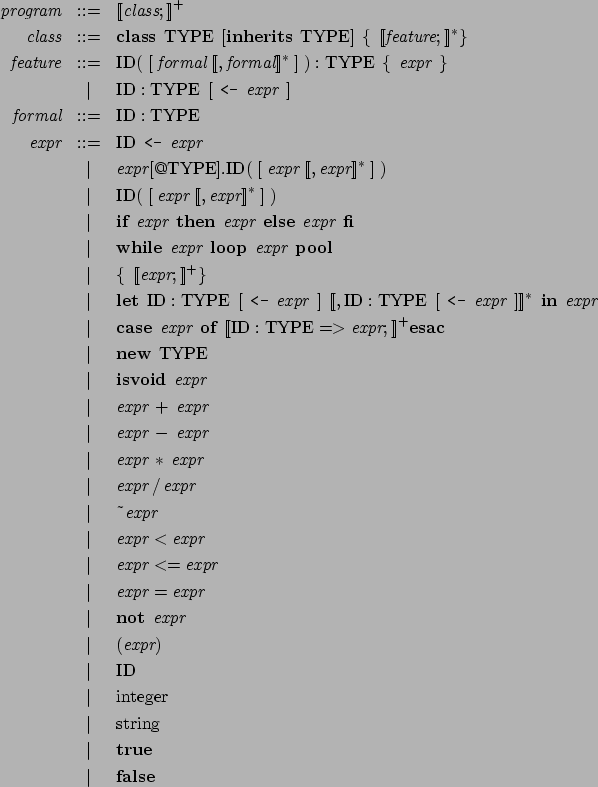
\includegraphics{img43.png}
\\\noalign{\medskip}
\hline
\noalign{\medskip}
\caption{\textbf{Figure 1:} Cool syntax.}
\end{longtable}

Figure~\hyperref[fig1]{1} provides a specification of Cool syntax. The
specification is not in pure Backus-Naur Form (BNF); for convenience, we
also use some regular expression notation. Specifically, $A^{\ast}$
means zero or more $A$'s in succession; $A^+$ means one or more $A$'s.
Items in square brackets $[\ldots]$ are optional. Double brackets
$\lbrack\!\lbrack \, \rbrack\!\rbrack $ are not part of Cool; they are
used in the grammar as a meta-symbol to show association of grammar
symbols (e.g. $a \lbrack\!\lbrack b c \rbrack\!\rbrack ^ {+}$ means $a$
followed by one or more $bc$ pairs).

\section{Getting Started}

Cool source files have extension \texttt{.cl}. The programming projects
will also define other file formats related to Cool but they are not
officially part of the language specification.

You can obtain the Cool interpreter \texttt{cool} from the course
website. To interpret (i.e., run) a Cool program:

\begin{verbatim}
cool file.cl 
\end{verbatim}

This official version is often called the \emph{reference
implementation} and you are encouraged to use it as a point of
comparison when you are designing and testing parts of the course
project.

The reference Cool interpreter has been specifically structured so that
you can run the various stages (i.e., lexing, parsing, type-checking and
interpreting) independently. This power is useful for PA2 through PA5.

The Cool interpreter has an number of command-line options:

\texttt{-{}-lex}

This option causes Cool to stop after lexing and produce a new file,
\texttt{file.cl-lex}, which contains the lexed tokens in a simple
interchange format. Handy for PA2.

\texttt{-{}-unlex}

This option causes Cool to undo lexing and produce \texttt{file.cl2} (a
Cool source file) from the lexed tokens. This is usually used as a
debugging aid for PA2 by feeding Cool a \texttt{file.cl-lex} file
produced by \emph{your lexer} from \texttt{file.cl} and then comparing
\texttt{file.cl2} to the original \texttt{file.cl}.

\texttt{-{}-parse}

This option causes Cool to stop after parsing and produce a new file,
\texttt{file.cl-ast}, which contains the abstract syntax tree in a
simple interchange format. Handy for PA3.

\texttt{-{}-unparse}

This option causes Cool to undo parsing and produce \texttt{file.cl3} (a
Cool source file) from the abstract syntax tree. This is usually used as
a debugging aid for PA3 by feeding Cool a \texttt{file.cl-ast} file
produced by \emph{your parser} from \texttt{file.cl} and then comparing
\texttt{file.cl3} to the original \texttt{file.cl}.

\texttt{-{}-type}

This option causes Cool to stop after type checking and semantic
analysis and produce a new file, \texttt{file.cl-type}, which contains
the \href{node47.html}{class mapping and implementation mapping} in a
simple interchange format. Handy for PA4.

\texttt{-{}-class-map}

This option causes Cool to stop after type checking and semantic
analysis and produce a new file, \texttt{file.cl-type}, which contains
the \href{node47.html}{class mapping} only in a simple interchange
format. Handy for the PA4 Checkpoint (WA4).

\texttt{-{}-imp-map}

This option causes Cool to stop after type checking and semantic
analysis and produce a new file, \texttt{file.cl-type}, which contains
the \href{node47.html}{implementation mapping} only in a simple
interchange format. Handy for the rest of PA4.

\texttt{-{}-out newname}

Causes Cool to produce \texttt{newname.cl} (or \texttt{.cl-ast}, or
whatever) instead of \texttt{file.cl}.

You may encounter other University uses of Cool on the web that mention
programs such as \texttt{coolc} and \texttt{spim}. Those tool are used
for a course on compilers; this is a course on interpreters. We will not
use \texttt{coolc} or \texttt{spim}. In addition, we use a slightly
different version of the Cool language specification, so comparing
results against external tools may not be helpful.

\subsection{Precedence}

The precedence of infix binary and prefix unary operations, from highest
to lowest, is given by the following table:

\begin{verbatim}
.
@
~
isvoid
* /
+ -
<=  <  =
not
<-
\end{verbatim}

All binary operations are left-associative, with the exception of
assignment, which is right-associative, and the three comparison
operations, which do not associate.

\section{Type Rules}

This section formally defines the type rules of Cool. The type rules
define the type of every Cool expression in a given context. The context
is the \emph{type environment}, which describes the type of every
unbound identifier appearing in an expression. The type environment is
described in Section~\href{node42.html\#sec-typenv}{12.1}.
Section~\href{node43.html\#sec-typr}{12.2} gives the type rules.

\subsection{Type Environments}

To a first approximation, type checking in Cool can be thought of as a
bottom-up algorithm: the type of an expression $e$ is computed from the
(previously computed) types of $e$'s subexpressions. For example, an
integer \texttt{1} has type \texttt{Int}; there are no subexpressions in
this case. As another example, if $\tt e_n$ has type $\tt X$, then the
expression $\tt\mbox {\tt\{}\ e_1; \ldots; e_n;\ \mbox {\tt\}}$ has type
$\tt X$.

A complication arises in the case of an expression $\tt v$, where
$\tt v$ is an object identifier. It is not possible to say what the type
of $\tt v$ is in a strictly bottom-up algorithm; we need to know the
type declared for $\tt v$ in the larger expression. Such a declaration
must exist for every object identifier in valid Cool programs.

To capture information about the types of identifiers, we use a
\emph{type environment}. The environment consists of three parts: a
method environment $M$, an object environment $O$, and the name of the
current class in which the expression appears. The method environment
and object environment are both functions (also called \emph{mappings}).
The object environment is a function of the form \\

\begin{displaymath}O(v) = T \end{displaymath}

which assigns the type $ T$ to object identifier $ v$. The method
environment is more complex; it is a function of the form \\

\begin{displaymath}M(C,f) = (T_1,\ldots,T_{n-1},T_n) \end{displaymath}

where $ C$ is a class name (a type), $f$ is a method name, and
$ t_1,\ldots,t_n$ are types. The tuple of types is the \emph{signature}
of the method. The interpretation of signatures is that in class $ C$
the method $f$ has formal parameters of types
$ (t_1,\ldots,t_{n-1})$--in that order--and a return type $t_n$.

Two mappings are required instead of one because object names and method
names do not clash--i.e., there may be a method and an object identifier
of the same name.

The third component of the type environment is the name of the current
class, which is needed for type rules involving \texttt{SELF\_TYPE}.

Every expression $e$ is type checked in a type environment; the
subexpressions of $e$ may be type checked in the same environment or, if
$e$ introduces a new object identifier, in a modified environment. For
example, consider the expression

\begin{verbatim}
  let c : Int <- 33 in
    ...
\end{verbatim}

The \texttt{let} expression introduces a new variable \texttt{c} with
type \texttt{Int}. Let 
\includegraphics{img56.png} be the object
component of the type environment for the \texttt{let}. Then the body of
the \texttt{let} is type checked in the object type environment \\

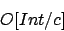
\includegraphics{img66.png}

where the notation 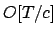
\includegraphics{img67.png} is defined as follows:

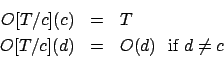
\includegraphics{img68.png}

\subsection{Type Checking Rules}

The general form a type checking rule is: \\

\begin{displaymath}
\frac{\vdots}{O,M,C \vdash e : T}\eqno\mbox{}
\end{displaymath}

The rule should be read: In the type environment for objects $O$,
methods $M$, and containing class $ C$, the expression $e$ has type
$ T$. The dots above the horizontal bar stand for other statements about
the types of sub-expressions of $e$. These other statements are
hypotheses of the rule; if the hypotheses are satisfied, then the
statement below the bar is true. In the conclusion, the
``\href{http://en.wikipedia.org/wiki/Turnstile_\%28symbol\%29}{turnstile}''
(``$\vdash$'') separates context ($O,M,C$) from statement ($e : T$).

The rule for object identifiers is simply that if the environment
assigns an identifier $ Id $ type $ T$, then $ Id $ has type $ T$. \\

\begin{displaymath}
\frac{O(Id) = T}{O,M,C \vdash Id : T}\eqno\mbox{[Var]}
\end{displaymath}

The rule for assignment to a variable is more complex: \\

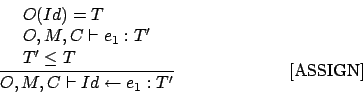
\includegraphics{img75.png}

Note that this type rule--as well as others--use the conformance
relation $\leq$ (see Section~\href{node6.html\#sec-inherit}{3.2}). The
rule says that the assigned expression $e_1$ must have a type $T'$ that
conforms to the type $ T$ of the identifier $ Id $ in the type
environment. The type of the whole expression is $T'$.

The type rules for constants are all easy: \\

\begin{displaymath}
\frac{}{O,M,C \vdash true : Bool}\eqno\mbox{[True]}
\end{displaymath}

\begin{displaymath}
\frac{}{O,M,C \vdash false : Bool}\eqno\mbox{[False]}
\end{displaymath}

\begin{displaymath}
\frac{i \mbox {\ is an integer constant}}{O,M,C \vdash i : Int}\eqno\mbox{[Int]}
\end{displaymath}

\begin{displaymath}
\frac{s \mbox {\ is a string constant}}{O,M,C \vdash s : String}\eqno\mbox{[String]}
\end{displaymath}

There are two cases for \texttt{new}, one for \texttt{new SELF\_TYPE}
and one for any other form: \\

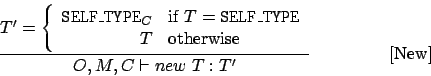
\includegraphics{img82.png}

Dispatch expressions are the most complex to type check. \\

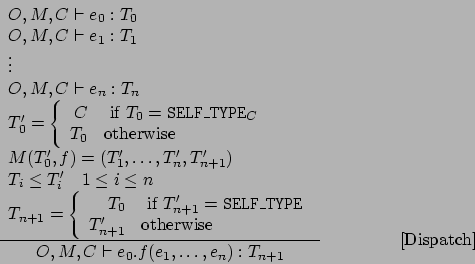
\includegraphics{img83.png}

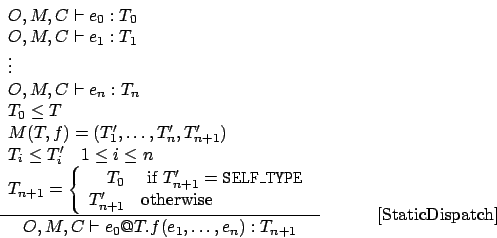
\includegraphics{img84.png}

To type check a dispatch, each of the subexpressions must first be type
checked. The type $T_0$ of $e_0$ determines which declaration of the
method $f$ is used. The argument types of the dispatch must conform to
the declared argument types. Note that the type of the result of the
dispatch is either the declared return type or $T_0$ in the case that
the declared return type is $\tt SELF\_TYPE$. The only difference in
type checking a static dispatch is that the class $ T$ of the method $f$
is given in the dispatch, and the type $T_0$ must conform to $ T$.

The type checking rules for \texttt{if} and \texttt{\{}-\texttt{\}}
expressions are straightforward. See
Section~\href{node18.html\#sec-cond}{7.5} for the definition of the

\includegraphics{img21.png} operation. \\

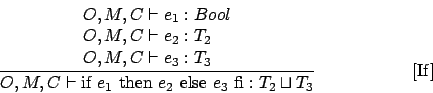
\includegraphics{img88.png}

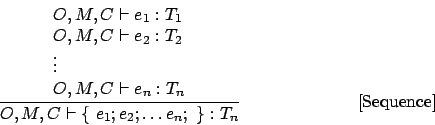
\includegraphics{img89.png}

The \texttt{let} rule has some interesting aspects. \\

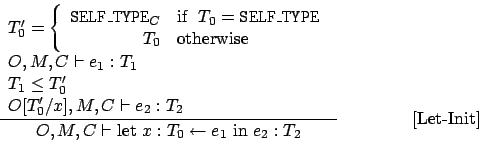
\includegraphics{img90.png}

First, the initialization 
\includegraphics{img76.png} is type checked in
an environment without a new definition for 
\includegraphics{img91.png}.
Thus, the variable 
\includegraphics{img91.png} cannot be used in

\includegraphics{img76.png} unless it already has a definition in an
outer scope. Second, the body 
\includegraphics{img92.png} is type
checked in the environment 
\includegraphics{img56.png} extended with the
typing 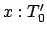
\includegraphics{img93.png}. Third, note that the type of

\includegraphics{img91.png} may be \texttt{SELF\_TYPE}.

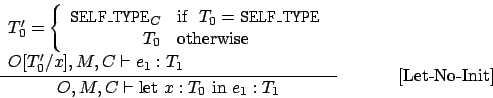
\includegraphics{img94.png}

The rule for \texttt{let} with no initialization simply omits the
conformance requirement. We give type rules only for a \texttt{let} with
a single variable. Typing a multiple \texttt{let} \\

\begin{displaymath}\rm let\ x_1 : T_1\ [\leftarrow e_1],\ x_2: T_2\ [\leftarrow e2], \ldots,\ x_n :T_n\ [\leftarrow e_n]\ in\ e\ \end{displaymath}

is defined to be the same as typing \\

\begin{displaymath}
\rm let\ x_1 : T_1\ [\leftarrow e_1]\ in\ (let\ x_2 :T_2\ [\leftarrow e_2],\ldots,\ x_n : T_n\ [\leftarrow e_n]\ in\ e\ )\
\end{displaymath}

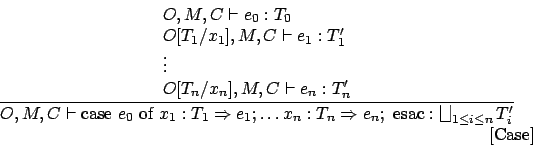
\includegraphics{img97.png}

Each branch of a \texttt{case} is type checked in an environment where
variable $x_i$ has type $T_i$. The type of the entire \texttt{case} is
the join of the types of its branches. The variables declared on each
branch of a \texttt{case} must all have distinct types.

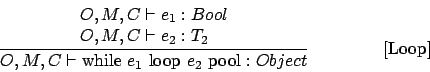
\includegraphics{img100.png}

The predicate of a loop must have type $Bool$; the type of the entire
loop is always $Object$. An \texttt{isvoid} test has type $Bool$: \\

\begin{displaymath}
\frac{O,M,C \vdash e_1 : T_1}{O,M,C \vdash \mbox {isvoid } e_1 : Bool}\eqno\mbox{[Isvoid]}
\end{displaymath}

With the exception of the rule for equality, the type checking rules for
the primitive logical and arithmetic operations are easy. \\

\begin{displaymath}
\frac{
O,M,C \vdash e_1 : Bool}{O,M,C \vdash \neg e_1 : Bool}\eqno\mbox{[Not]}
\end{displaymath}

\begin{displaymath}
\frac{
O,M,C \vdash e_1 : Int}{O,M,C \vdash \mbox{\~{}} e_1 : Int}\eqno\mbox{[Neg]}
\end{displaymath}

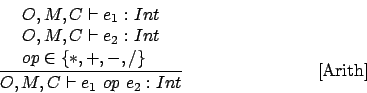
\includegraphics{img107.png}

The wrinkle in the rule for equality is that any types may be freely
compared except \texttt{Int, String} and \texttt{Bool}, which may only
be compared with objects of the same type. The cases for
\texttt{\textless{}} and \texttt{\textless{}=} are similar to the rule
for equality. \\

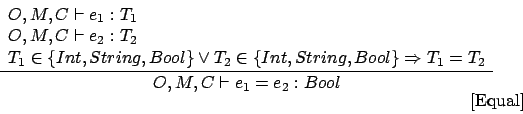
\includegraphics{img108.png}

The final cases are type checking rules for attributes and methods. For
a class 
\includegraphics{img61.png}, let the object environment

\includegraphics{img109.png} give the types of all attributes of

\includegraphics{img61.png} (including any inherited attributes). More
formally, if 
\includegraphics{img91.png} is an attribute (inherited or
not) of 
\includegraphics{img61.png}, and the declaration of

\includegraphics{img91.png} is \includegraphics{img110.png}, then \\

\includegraphics{img111.png}

The method environment \includegraphics{img55.png} is global to the
entire program and defines for every class \includegraphics{img61.png}
the signatures of all of the methods of \includegraphics{img61.png}
(including any inherited methods).

The two rules for type checking attribute defininitions are similar the
rules for \texttt{let}. The essential difference is that attributes are
visible within their initialization expressions. Note that \texttt{self}
is bound in the initialization. \\

\includegraphics{img112.png}

\includegraphics{img113.png}

The rule for typing methods checks the body of the method in an
environment where \includegraphics{img109.png} is extended with bindings
for the formal parameters and \texttt{self}. The type of the method body
must conform to the declared return type.

\includegraphics{img114.png}

\subsection{Other Semantic Checks}

There are a number of semantic checks applied to Cool programs that are
not captured by formal typing rules. For example, a Cool program cannot
contain an inheritance cycle. Similarly, a Cool program cannot contain a
class that inherits from \texttt{String}. These rules are scattered
through the \emph{Cool Reference Manual}.

The order in which these other checks are performed is \emph{not
specified}. If a Cool program contains both an inheritance cycle and
also a class htat inherits from \texttt{String}, the Cool compiler may
report whichever error it prefers.

\section{Operational Semantics}

This section contains a mostly formal presentation of the operational
semantics for the Cool language. The operational semantics define for
every Cool expression what value it should produce in a given context.
The context has three components: an environment, a store, and a self
object. These components are described in the next section. Section
\href{node46.html\#objectsyntax}{13.2} defines the syntax used to refer
to Cool objects, and Section \href{node47.html\#classdefs}{13.3} defines
the syntax used to refer to class definitions.

Keep in mind that a formal semantics is a specification only--it does
not describe an implementation. The purpose of presenting the formal
semantics is to make clear all the details of the behavior of Cool
expressions. How this behavior is implemented is another matter.

\subsection{Environment and the Store}

Before we can present a semantics for Cool we need a number of concepts
and a considerable amount of notation. An \emph{environment} is a
mapping of variable identifiers to \emph{locations}. Intuitively, an
environment tells us for a given identifier the address of the memory
location where that identifier's value is stored. For a given
expression, the environment must assign a location to all identifiers to
which the expression may refer. For the expression, e.g., $a + b$, we
need an environment that maps $a$ to some location and $b$ to some
location. We'll use the following syntax to describe environments, which
is very similar to the syntax of type assumptions used in
Section~\href{node41.html\#sec-typrules}{12}. \\

\begin{displaymath}
E = [ a:l_1, b:l_2]
\end{displaymath}

This environment maps $a$ to location $l_1$, and $b$ to location $l_2$.

The second component of the context for the evaluation of an expression
is the \emph{store} (memory). The store maps locations to values, where
values in Cool are just objects. Intuitively, a store tells us what
value is stored in a given memory location. For the moment, assume all
values are integers. A store is similar to an environment: \\

\begin{displaymath}
S = [ l_1\rightarrow 55, l_2\rightarrow 77 ]
\end{displaymath}

This store maps location $l_1$ to value $55$ and location $l_2$ to value
$77$.

Given an environment and a store, the value of an identifier can be
found by first looking up the location that the identifier maps to in
the environment and then looking up the location in the store. \\

\begin{displaymath}
\begin{array}{rcl}
E(a) &=& l_1 \\
S(l_1) & = & 55
\end{array}\end{displaymath}

Together, the environment and the store define the execution state at a
particular step of the evaluation of a Cool expression. The double
indirection from identifiers to locations to values allows us to model
variables. Consider what happens if the value $99$ is assigned variable
$a$ in the environment and store defined above. Assigning to a variable
means changing the value to which it refers but not its location. To
perform the assignment, we look up the location for $a$ in the
environment $E$ and then change the mapping for the obtained location to
the new value, giving a new store $S'$.

\begin{displaymath}
\begin{array}{rcl}
E(a) & = & l_1 \\
S' & = & S[99/l_1]
\end{array}\end{displaymath}

The syntax $S[v/l]$ denotes a new store that is identical to the store
$S$, except that $S'$ maps location $l$ to value $ v$. For all locations
$l'$ where $l'\not=l$, we still have $S'(l')=S(l')$.

The store models the contents of memory of the computer during program
execution. Assigning to a variable modifies the store.

There are also situations in which the environment is modified. Consider
the following Cool fragment:

\begin{verbatim}
  let c : Int <- 33 in
    c
\end{verbatim}

When evaluating this expression, we must introduce the new identifier
$c$ into the environment before evaluating the body of the \texttt{let}.
If the current environment and state are $E$ and $S$, then we create a
new environment $E'$ and a new store $S'$ defined by: \\

\begin{displaymath}
\begin{array}{rcl}
l_c & = & newloc(S)\\
E' & = & E[l_c/c]\\
S' & = & S[33/l_c]
\end{array}\end{displaymath}

The first step is to allocate a location for the variable $c$. The
location should be fresh, meaning that the current store does not have a
mapping for it. The function $newloc()$ applied to a store gives us an
unused location in that store. We then create a new environment $E'$,
which maps $c$ to $l_c$ but also contains all of the mappings of $E$ for
identifiers other than $c$. Note that if $c$ already has a mapping in
$E$, the new environment $E'$ hides this old mapping. We must also
update the store to map the new location to a value. In this case $l_c$
maps to the value $33$, which is the initial value for $c$ as defined by
the let-expression.

The example in this subsection oversimplifies Cool environments and
stores a bit, because simple integers are not Cool values. Even integers
are full-fledged objects in Cool.

\subsection{Syntax for Cool Objects}

Every Cool value is an object. Objects contain a list of named
attributes, a bit like records in C. In addition, each object belongs to
a class. We use the following syntax for values in Cool: \\

\begin{displaymath}
v = X(a_1=l_1,a_2=l_2,\ldots,a_n=l_n)
\end{displaymath}

Read the syntax as follows: The value $ v$ is a member of class $X$
containing the attributes $a_1, \ldots, a_n$ whose locations are
$l_1, \ldots, l_n$. Note that the attributes have an associated
location. Intuitively this means that there is some space in memory
reserved for each attribute. The value $ v$ has \emph{dynamic} type $X$.

For base objects of Cool (i.e., \texttt{Int}s, \texttt{String}s, and
\texttt{Bool}s) we use a special case of the above syntax. Base objects
have a class name, but their attributes are not like attributes of
normal classes, because they cannot be modified. Therefore, we describe
base objects using the following syntax:

\begin{displaymath}
\begin{array}{l}
Int(5)\\
Bool(true)\\
String(4,\mbox {\tt ''}Cool \mbox {\tt ''})
\end{array}\end{displaymath}

For \texttt{Int}s and \texttt{Bool}s, the meaning is obvious.
\texttt{String}s contain two parts, the length and the actual sequence
of ASCII characters.

\subsection{Class definitions}

In the rules presented in the next section, we need a way to refer to
the definitions of attributes and methods for classes. Suppose we have
the following Cool class definition:

\begin{verbatim}
   class B {
      s : String <- "Hello";
      g (y:String) : Int {
         y.concat(s)
      };
      f (x:Int) : Int {
         x+1
      };
   };

   class A inherits B {
      a : Int;
      b : B <- new B;
      f(x:Int) : Int {
         x+a
      };
   };
\end{verbatim}

Two mappings, called \emph{class} and \emph{implementation}, are
associated with class definitions. The \emph{class} mapping is used to
get the attributes, as well as their types and initializations, of a
particular class: \\

\includegraphics{img145.png}

Note that the information for class \includegraphics{img45.png} contains
everything that it inherited from class \includegraphics{img146.png}, as
well as its own definitions. If \includegraphics{img146.png} had
inherited other attributes, those attributes would also appear in the
information for \includegraphics{img45.png}. The attributes are listed
in the order they are inherited and then in source order: all the
attributes from the greatest ancestor are listed first in the order in
which they textually appear, then the attributes of the next greatest
ancestor, and so on, on down to the attributes defined in the particular
class. We rely on this order in describing how new objects are
initialized.

The general form of a class mapping is: \\

\includegraphics{img147.png}

Note that every attribute has an initializing expression, even if the
Cool program does not specify one for each attribute. The default
initialization for a variable or attribute is the \emph{default} of its
type. The default of \texttt{Int} is 0, the default of \texttt{String}
is \includegraphics{img148.png}, the default of \texttt{Bool} is
\texttt{false}, and the default of any other type is
\texttt{void}.\href{footnode.html\#foot1803}{\textsuperscript{5}}The
default of type \includegraphics{img58.png} is written
\includegraphics{img149.png}.

The implementation mapping gives information about the methods of a
class. For the above example, \emph{implementation} of A is defined as
follows:

\includegraphics{img150.png}

In general, for a class \includegraphics{img141.png} and a method
\includegraphics{img151.png}, \\

\includegraphics{img152.png}

specifies that method \includegraphics{img151.png} when invoked from
class \includegraphics{img141.png}, has formal parameters
\includegraphics{img153.png}, and the body of the method is expression
\includegraphics{img154.png}.

\subsection{Operational Rules}

Equipped with environments, stores, objects, and class definitions, we
can now attack the operational semantics for Cool. The operational
semantics is described by rules similar to the rules used in type
checking. The general form of the rules is: \\

\begin{displaymath}
\frac{\vdots}{so,S,E\vdash e_1 : v,S'}\eqno
\mbox{}
\end{displaymath}

The rule should be read as: In the context where \emph{self} is the
object $so$, the store is $S$, and the environment is $E$, the
expression $e_1$ evaluates to object $ v$ and the new store is $S'$. The
dots above the horizontal bar stand for other statements about the
evaluation of sub-expressions of $e_1$.

Besides an environment and a store, the evaluation context contains a
self object $so$. The self object is just the object to which the
identifier \texttt{self} refers if \texttt{self} appears in the
expression. We do not place \texttt{self} in the environment and store
because \texttt{self} is not a variable--it cannot be assigned to. Note
that the rules specify a new store after the evaluation of an
expression. The new store contains all changes to memory resulting as
side effects of evaluating expression $e_1$.

The rest of this section presents and briefly discusses each of the
operational rules. A few cases are not covered; these are discussed at
the end of the section. \\

\includegraphics{img157.png}

An assignment first evaluates the expression on the right-hand side,
yielding a value $v_1$. This value is stored in memory at the address
for the identifier.

The rules for identifier references, \texttt{self}, and constants are
straightforward: \\

\includegraphics{img159.png}

\includegraphics{img160.png}

\includegraphics{img161.png}

\includegraphics{img162.png}

\includegraphics{img163.png}

\includegraphics{img164.png}

A \texttt{new} expression is more complicated than one might expect: \\

\includegraphics{img165.png}

The tricky thing in a \texttt{new} expression is to initialize the
attributes in the right order. If an attribute does not have an
initializer, \emph{do not} evaluate an assignment expression for it in
the final step. Note also that, during initialization, attributes are
bound to the default of the appropriate class.

\includegraphics{img166.png}

\includegraphics{img167.png}

The two dispatch rules do what one would expect. The arguments are
evaluated and saved. Next, the expression on the left-hand side of the
``.'' is evaluated. In a normal dispatch, the class of this expression
is used to determine the method to invoke; otherwise the class is
specified in the dispatch itself.

\includegraphics{img168.png}

\includegraphics{img169.png}

There are no surprises in the if-then-else rules. Note that value of the
predicate is a \texttt{Bool} object, not a boolean.

\includegraphics{img170.png}

Blocks are evaluated from the first expression to the last expression,
in order. The result is the result of the last expression.

\includegraphics{img171.png}

A \texttt{let} evaluates any initialization code, assigns the result to
the variable at a fresh location, and evaluates the body of the
\texttt{let}. (If there is no initialization, the variable is
initialized to the default value of \includegraphics{img172.png}.) We
give the operational semantics only for the case of \texttt{let} with a
single variable. The semantics of a multiple \texttt{let} \\

\includegraphics{img173.png}

is defined to be the same as \\

\includegraphics{img174.png}

\includegraphics{img175.png}

Note that the \texttt{case} rule requires that the class hierarchy be
available in some form at runtime, so that the correct branch of the
\texttt{case} can be selected. This rule is otherwise straightforward.
\\

\includegraphics{img176.png}

\includegraphics{img177.png}

There are two rules for \texttt{while}: one for the case where the
predicate is \texttt{true} and one for the case where the predicate is
\texttt{false}. Both cases are straightforward. The two rules for
\texttt{isvoid} are also straightforward: \\

\includegraphics{img178.png}

\includegraphics{img179.png}

The remainder of the rules are for the primitive arithmetic and logical
operations. These are all easy rules. \\

\includegraphics{img180.png}

\includegraphics{img182.png}

\includegraphics{img183.png}

Cool \texttt{Int}s are 32-bit two's complement signed integers; the
arithmetic operations are defined accordingly.

The notation and rules given above are not powerful enough to describe
how objects are tested for equality, or how runtime exceptions are
handled. For these cases we resort to an English description.

In $e_1 = e_2$, first $e_1$ is evaluated and then $e_2$ is evaluated.
The two objects are compared for equality by first comparing their
pointers (addresses). If they are the same, the objects are equal. The
value \texttt{void} is not equal to any object except itself. If the two
objects are of type \texttt{String}, \texttt{Bool}, or \texttt{Int},
their respective contents are compared. \texttt{\textless{}} and
\texttt{\textless{}=} are handled similarly. The case for integer
arguments is simple:

\includegraphics{img181.png}

\ldots{} but \texttt{String} and \texttt{Bool} also admit comparisons.
String comparisons are performed using the standard ASCII string
ordering (e.g., \texttt{"abc" \textless{} "xyz"}). For booleans,
\texttt{false} is defined to be less than \texttt{true}. Any other
comparison (e.g., a comparison among non-void objects of different
types) returns \texttt{false}. Note that for some objects this may be
unintuitive: if \texttt{c} is a \texttt{Cat} and \texttt{d} is a
\texttt{Dog} then \texttt{c \textless{} d} is \texttt{false} but
\texttt{d \textless{} c} is \emph{also} \texttt{false}. Note also that
comparison is based on the dynamic type of the object, not on the static
type of the object.

In addition, the operational rules do not specify what happens in the
event of a runtime error. When a runtime error occurs, output is flushed
and execution aborts. The following list specifies all possible runtime
errors.

\begin{enumerate}
\itemsep1pt\parskip0pt\parsep0pt
\item
  A dispatch (static or dynamic) on \texttt{void}.
\item
  A case on \texttt{void}.
\item
  Execution of a case statement without a matching branch.
\item
  Division by zero.
\item
  Substring out of range. \emph{(This error is always reported on line
  0, since it occurs inside an ``internal'' library function.)}
\item
  Heap overflow. \emph{(You do not need to implement this runtime
  error.)}
\item
  Stack overflow.
\end{enumerate}

Each outstanding ``method invocation'' (static or dynamic) and each
outstanding ``new'' object allocation expression counts as a ``Cool
Activation Record''. (Just to be clear, that second clause about ``new''
is counting currently-resolving constructor calls, not ``total objects
living in the heap''.) A Cool interpreter \emph{must} flag a ``stack
overflow'' runtime error if and only if there are \textbf{1000} (one
thousand) or more outstanding Cool Activation Records.

Finally, the rules given above do not explain the execution behaviour
for dispatches to primitive methods defined in the \texttt{Object},
\texttt{IO}, or \texttt{String} classes. Descriptions of these primitive
methods are given in
Sections~\href{node29.html\#sec-int}{8.3}-\href{node31.html\#sec-bool}{8.5}.

\section{Acknowledgements}

Cool is based on Sather164, which is itself based on the language
Sather. Portions of this document were cribbed from the Sather164
manual; in turn, portions of the Sather164 manual are based on Sather
documentation written by Stephen M. Omohundro.

A number people have contributed to the design and implementation of
Cool, including Manuel Fähndrich, David Gay, Douglas Hauge, Megan
Jacoby, Tendo Kayiira, Carleton Miyamoto, and Michael Stoddart. Joe
Darcy updated Cool to the current version.

This version (used in Virginia CS 415) of Cool owes a great debt to
George C. Necula and Bor-Yuh Evan Chang.


\section{Classes}

All code in Cool is organized into classes. Each class definition must
be contained in a single source file, but multiple classes may be
defined in the same file. Class definitions have the form:

\begin{verbatim}
class <type> [ inherits <type> ] {
    <feature_list>
};
\end{verbatim}

The notation \texttt{{[} ...{]}} denotes an optional construct. All
class names are globally visible. Class names begin with an uppercase
letter. Classes may not be redefined.

\section{About this document \ldots{}}

\textbf{The Cool Reference
Manual\href{footnode.html\#foot266}{\textsuperscript{1}}}

\section{Cool Assembly Language}

Cool Assembly Language is a simplified RISC-style assembly language that
is reminiscient of
\href{http://en.wikipedia.org/wiki/MIPS_architecture\#MIPS_assembly_language}{MIPS
Assembly Language} crossed with
\href{http://en.wikipedia.org/wiki/X86_assembly_language}{x86 Assembly
Language}. It also features typing aspects that may remind one of
\href{http://en.wikipedia.org/wiki/Java_bytecode}{Java Bytecode}.

A Cool Assembly Language \textbf{program} is a list of
\textbf{instructions}. Each instruction may be preceeded by any number
of \textbf{labels}. Comments follow the standard Cool conventions. In
addition, a semicolon \texttt{;} functions like a double dash
\texttt{-{}-} in that it marks the rest of that line as a comment. The
Cool CPU is a \href{http://en.wikipedia.org/wiki/RISC}{load-store
architecture} with eight
\href{http://en.wikipedia.org/wiki/General_purpose_register}{general
purpose registers} and three special-purpose registers. For simplicity,
a machine word can hold either a 32-bit integer value or an entire raw
string; regardless, all machine words have size one.

This document assumes that you already have some familiarity with
assembly language, registers, and how CPUs operate. We first present a
formal grammar and then explain the semantics. Only terms in
\texttt{typewriter font} are part of the formal grammar. Text after ---
is a comment. We use \texttt{italics} for non-terminals.

\texttt{register ::= r0} --- general purpose register \#0, often used as
the \emph{accumulator}\\ \texttt{register ::= r1} --- general purpose
register \#1 \\ \texttt{register ::= r2}\\ \texttt{register ::= r3}\\
\texttt{register ::= r4}\\ \texttt{register ::= r5}\\
\texttt{register ::= r6}\\ \texttt{register ::= r7}\\
\texttt{register ::= sp} --- stack pointer register\\
\texttt{register ::= fp} --- frame pointer register\\
\texttt{register ::= ra} --- return address register\\

\texttt{instruction ::= li  register \textless{}- integer} --- load
immediate \\ \texttt{instruction ::= mov register \textless{}- register}
--- register-to-register copy \\
\texttt{instruction ::= add register \textless{}- register register}\\
\texttt{instruction ::= sub register \textless{}- register register}\\
\texttt{instruction ::= mul register \textless{}- register register}\\
\texttt{instruction ::= div register \textless{}- register register}\\

\texttt{instruction ::= jmp label } --- unconditional branch\\
\texttt{instruction ::= bz register label } --- branch if equal to zero
\\ \texttt{instruction ::= bnz register label } --- branch if not zero
\\ \texttt{instruction ::= beq register register label } --- branch if
equal \\ \texttt{instruction ::= blt register register label } ---
branch if less than \\
\texttt{instruction ::= ble register register label } --- branch if less
than or equal to \\ \texttt{instruction ::= call label } --- direct
function call\\ \texttt{instruction ::= call register } ---
register-indirect function call\\ \texttt{instruction ::= return } ---
function return\\

\texttt{instruction ::= push register } --- push a value on the stack\\
\texttt{instruction ::= pop register } --- push a value off the stack\\
\texttt{instruction ::= ld register \textless{}- register {[} integer {]} }
--- load a value from memory \\
\texttt{instruction ::= st register {[} integer {]} \textless{}- register }
--- store a value into memory \\
\texttt{instruction ::= la register \textless{}- label } --- load an
address into a register \\

\texttt{instruction ::= alloc register register } --- allocate memory\\
\texttt{instruction ::= constant integer } --- lay out a compile-time
constant in memory\\ \texttt{instruction ::= constant raw\_string } ---
lay out a compile-time constant in memory\\
\texttt{instruction ::= constant label } --- lay out a compile-time
constant in memory\\

\texttt{instruction ::= syscall name } --- request a service from the
run-time system\\

\texttt{instruction ::= debug register } --- debugging support: print
register value \\ \texttt{instruction ::= trace } --- toggle tracing \\

That's it, and the last two do not really count. We next describe the
interpretation of these instructions in more detail.

\begin{itemize}
\itemsep1pt\parskip0pt\parsep0pt
\item
  Note that there are only eight general purpose registers available, as
  with the x86 instruction set. This is a departure from general RISC,
  but it will give you more of a feel for the real world. Eight is
  entirely sufficient for a stack-machine style of code generation --
  the reference compiler only uses four of them. However, for advanced
  optimizations such as register allocation, eight is quite small.
\item
  \texttt{li r1 \textless{}- some\_int} overwrites \texttt{r1} with a
  the value \texttt{some\_int}
\item
  Note that in Cool Assembly Language, the arrows \texttt{\textless{}-}
  are required. They remind you that the destination is always on the
  left and the operands are always on the right.
\item
  \texttt{bz r1 label} jumps to \texttt{label} if the value of
  \texttt{r1} is zero. If not, control passes to the instruction
  immediately following this one.
\item
  \texttt{beq r1 r2 label} jumps to \texttt{label} if the registers
  \texttt{r1} and \texttt{r2} hold the same value.
\item
  \texttt{ble r1 r2 label} jumps to \texttt{label} if the value of
  \texttt{r1} is less than or equal to the value of \texttt{r2}. For
  integers this is standard. If \texttt{r1} and \texttt{r2} hold raw
  strings, those strings are compared lexicographically.
\item
  \texttt{call label} stores the value of the next instruction (i.e.,
  the value of the current program counter + 1) in the \texttt{ra}
  register and then jumps to \texttt{label}.
\item
  \texttt{call register} stores the value of the next instruction (i.e.,
  the value of the current program counter + 1) in the \texttt{ra}
  register and then jumps to address stored in \emph{register}.
\item
  \texttt{return} jumps to the address stored in the \texttt{ra}
  register.
\item
  Like the x86, the Cool CPU has explicit support for a stack. The stack
  pointer starts at a very high value and \emph{grows down}, toward
  smaller numbers, as values are pushed on it. \texttt{push r1} takes
  the value of \texttt{r1} and stores it at the address given by the
  stack pointer \texttt{sp} and then decrements \texttt{sp}.
  \texttt{pop   r1} increments \texttt{sp} and then loads the value from
  the address given by the stack pointer and copies that value into
  \texttt{r1}.
\item
  \texttt{ld r1 \textless{}- r2 {[} offset {]} } computes an address by
  adding \texttt{offset} to the value stored in \texttt{r2}. The
  contents of that address are loaded and written to \texttt{r1}.
\item
  \texttt{st r1 {[} offset {]} \textless{}- r2 } computes an address by
  adding \texttt{offset} to the value stored in \texttt{r1}. The
  contents of \texttt{r2} are stored into that address in memory.
\item
  \texttt{la r1 label} stores the address associated with \texttt{label}
  into \texttt{r1}.
\item
  \texttt{alloc r1 r2} allocates new contiguous memory and stores a
  pointer to it in \texttt{r1}. The number of words to be allocated is
  given in \texttt{r2}. For example, if \texttt{r2 = 5} and
  \texttt{alloc r1   r2} assigns \texttt{100} into \texttt{r1}, then
  \texttt{100} through \texttt{104} are now valid memory addresses.
\item
  \texttt{constant whatever} lays out \texttt{whatever} in program
  memory before execution begins.
\end{itemize}

The system calls available are:

\begin{itemize}
\itemsep1pt\parskip0pt\parsep0pt
\item
  \texttt{syscall IO.in\_string} reads a raw string from the user,
  allocates one word of memory, stores the raw string value in that
  memory word, and then stores the address of that memory word in
  \texttt{r1}. Note that this yields a raw string value and not a Cool
  String object -- you'll have to do a bit more work to package it up
  into a full-fledged Cool String object.
\item
  \texttt{syscall IO.in\_int} reads an integer from the user and stores
  that integer value in \texttt{r1}. Note that this yields a raw integer
  value and not a Cool Int object.
\item
  \texttt{syscall IO.out\_int} reads the value in \texttt{r1} and
  displays it as an integer to the user. Note that \texttt{r1} should be
  a raw integer and not an entire large Cool Int object.
\item
  \texttt{syscall IO.out\_string} reads the value in \texttt{r1}, which
  should be an address that points to a machine word containing a raw
  string. That raw string value is read from memory and displayed to the
  user. Note that \texttt{r1} should be a pointer to a raw string, and
  not a large Cool String object.
\item
  \texttt{syscall String.length} reads the value in \texttt{r1}, which
  should be an address that points to a machine word containing a raw
  string. The length of that string value is computed and stored in
  \texttt{r1}.
\item
  \texttt{syscall String.concat} reads the values in \texttt{r1} and
  \texttt{r2}, both of which should be addresses that point to machine
  words that contain raw strings. A machine word for a new string is
  allocated in memory. That new string contains the r1-string
  concatenated with the r2-string. The register \texttt{r1} is
  overwritten so that it contains a pointer to the newly-created raw
  string.
\item
  \texttt{syscall String.substr} reads the value in \texttt{r0}, which
  should be an address that points to a machine word containing a raw
  string, as well as \texttt{r1} and \texttt{r2}, which are both raw
  integer values.

  \begin{itemize}
  \itemsep1pt\parskip0pt\parsep0pt
  \item
    If r1\textless{}0, r2\textless{}0, or r1+r2\textgreater{} the length
    of the raw string, the system call stores 0 in \texttt{r1}.
  \item
    Otherwise, a word is allocated in memory to hold a new raw string.
    That new raw string holds the substring specified by the three
    arguments. The address of that new raw string is stored in
    \texttt{r1}.
  \end{itemize}
\item
  \texttt{syscall exit} terminates execution of the Cool Assembly
  Language program.
\end{itemize}

That system calls correspond directly to internal predefined methods on
Cool Int and String objects. The key difference is that the system calls
work on raw values (i.e., machine-level ints and strings) and not on
Cool Objects.

\section{Cool CPU Simulator}

The normal Cool compiler executable (e.g., \texttt{cool.exe}) also
serves as a Cool CPU Simulator that executes Cool Assembly Language
programs. Just pass \texttt{file.cl-asm} as an argument.

The simulator performs the following actions:

\begin{enumerate}
\itemsep1pt\parskip0pt\parsep0pt
\item
  Load the \texttt{.cl-asm} program into memory starting at address
  1000. That is, if the first instruction in \texttt{file.cl-asm} is
  \texttt{mov r1, r2}, then memory location 1000 will hold the
  instruction \texttt{mov r1, r2}. If the second instruction in
  \texttt{file.cl-asm} is \texttt{constant 55}, then memory location
  1001 will hold the integer 55.
\item
  Set \texttt{sp} and \texttt{fp} to 2,000,000,000. Remember, the stack
  starts at high addresses and grows down.
\item
  Search \texttt{file.cl-asm} for a label named \texttt{start}. The
  program counter is set to the address corresponding to that label. For
  example, if \texttt{start:} occurs just before the third instruction
  in \texttt{file.cl-asm}, then the program counter starts at 1002.
\item
  Fetch the instruction pointed to by the program counter and execute
  it. Unless the instruction specifies otherwise, the program counter is
  incremented by one and the process repeats.
\item
  When memory is allocated (e.g., by the \texttt{alloc} instruction),
  addresses starting from at least 20,000 are used.
\item
  If more than 1000 \texttt{call} instructions are executed before any
  \texttt{return} instructions are executed (i.e., if there are more
  than 1000 calls on the stack), the simulator terminates and prints a
  stack overflow error.
\end{enumerate}

The constant values listed above (1000; 20,000; 2,000,000,000) should
not be counted on by your program, but are listed here to help with
debugging. Addresses near 1000 hold program instructions or compile-time
data (i.e., the code segment), addresses near 20,000 hold the heap, and
addresses near two billion are on the stack.

\section{Debugging}

Debugging assembly language programs is notoriously difficult! While
writing your code generator, you will spend quite a bit of time running
generated Cool Assembly programs through the Cool CPU Simulator to see
if they work. Often they will not. The Cool CPU Simulator has been
designed with a large number of features to aid debugging. Basically
none of these features are present in traditional assemblers, so you
actually have a wealth of debugging support, but it will still be
difficult.

\begin{itemize}
\itemsep1pt\parskip0pt\parsep0pt
\item
  The simulator tracks a notion of time --- the first instruction is
  executed at time one, the second at time two, etc. More importantly:
\item
  The simulator tracks, for each register and memory value, the last
  time it was written to and the instruction that wrote to it. This can
  be invaluable for tracking down memory corruption errors (e.g.,
  finding who is scribbling over memory) or otherwise determining why
  \texttt{r1} holds an integer when you were sure it was supposed to
  hold a string.
\item
  If you try to read from a register or a memory address that has never
  been written to, the simulator will catch it and abort the program,
  rather than continuing with a garbage value.
\item
  You can use the \texttt{debug r1} opcode to print out the current
  value of any register, as well as its last modification information.
\item
  The simulator keeps track of integers, strings, labels and code
  segment addresses separately ``under the hood''. Thus if you execute
  \texttt{la r5 my\_label} and then inspect the value of \texttt{r5}, it
  will print as \texttt{label my\_label} rather than \texttt{1056} or
  whatever that address happens to be. This can be quite handy for
  tracking down problems related to virtual function tables. Perhaps
  more importantly:
\item
  The simulator uses this type information when simulating instructions,
  and stops early if you provide the wrong type of argument. For
  example, in \texttt{st r1 {[} 0 {]} \textless{}- r2}, if \texttt{r1}
  is actually a string or a pointer to the code segment, the simulator
  will raise an error rather than silently corrupting your program. If
  \texttt{r1} is a label or integer address, everything works fine. (If
  the string example confuses you, remember that in Cool Assembly
  Language a raw string is a one-word value that fits in a register, not
  a C-style pointer to a buffer.)
\item
  The simulator keeps a best effort stack trace. If you use the
  \texttt{call} and \texttt{return} instructions, the simulator will
  keep track of which functions were called, and from where, and print
  that back trace out if there is an error.
\item
  When dynamically allocating memory, the simulator actually allocates
  more space than is needed and leaves the remainder empty. For example,
  if you make two allocations of five words each, you may get back the
  addresses 21,000 and 21,010. The range 21,005-21,009 remains unused,
  and if you attempt to read from it, the simulator will abort. This can
  help to prevent walking off the end of a buffer.
\item
  If you attempt to divide by zero or dereference a null pointer, the
  simulator will catch it.
\item
  Finally, if you use the \texttt{-{}-trace-eval} option to
  \texttt{cool.exe} or execute the \texttt{trace} instruction (which
  toggles the state of tracing), the simulator will print copious
  debugging information before every time step, including the contents
  of all registers and the current instruction.
\end{itemize}

\section{Control Flow Graphs}

The Cool reference compiler also includes options to produce control
flow graphic visualizations in the style of the \texttt{dotty} tool from
the \href{http://en.wikipedia.org/wiki/Graphviz}{Graphviz} toolkit.

Passing the \texttt{-{}-cfg} option (with, for example,
\texttt{-{}-opt -{}-asm}) produces \texttt{method.dot}, which can then
be inspected via a number of tools. For example, this program:

\begin{verbatim}
class Main {
  main():Object {
    if (isvoid self) then  
      (new IO).out_string("cannot happen!\n")
    else 
      (new IO).out_string("hello, world!\n")
    fi 
  };
};
\end{verbatim}

Might produce this control-flow graph:

\includegraphics{cfg-example.png}

While you do not have to match the reference compiler exactly,
inspecting its control-flow graphs can help you debug your own code to
create control-flow graphs.

\section{Performance Model}

As discussed above, the Cool reference compiler also includes a
reference machine simulator to interpret Cool Assembly Language
instructions. This simulator can be invoked directly by passing a
\texttt{.cl-asm} file to \texttt{cool.exe}:

\begin{verbatim}
cool$ cat hello-world.cl
class Main {
  main():Object {
    (new IO).out_string("hello, world!\n")
  };
};
cool$ ./cool --asm hello-world.cl
cool$ ./cool hello-world.cl-asm 
hello, world!
\end{verbatim}

The simulator can also give detailed performance information:

\begin{verbatim}
 
cool$ ./cool --profile hello-world.cl-asm 
hello, world!
PROFILE:           instructions =        107 @    1 =>        107
PROFILE:        pushes and pops =         29 @    1 =>         29
PROFILE:             cache hits =         22 @    0 =>          0
PROFILE:           cache misses =        570 @  100 =>      57000
PROFILE:     branch predictions =          0 @    0 =>          0
PROFILE:  branch mispredictions =         11 @   20 =>        220
PROFILE:        multiplications =          0 @   10 =>          0
PROFILE:              divisions =          0 @   40 =>          0
PROFILE:           system calls =          2 @ 1000 =>       2000
CYCLES: 59356
\end{verbatim}

The execution time of a Cool Assembly Language program is measured in
simulated \href{http://en.wikipedia.org/wiki/CPU_cycle}{instruction
cycles}. In general, each assembly instruction takes one cycle. Some
instructions, such as system calls or memory operation, can cost many
more cycles. The total cycle cost of a program is the sum of all of its
component cycle costs.

In modern architectures,
\href{http://en.wikipedia.org/wiki/Memory_hierarchy}{memory hierarchy}
effects (e.g., \href{http://en.wikipedia.org/wiki/Cache}{caching}) and
\href{http://en.wikipedia.org/wiki/Branch_prediction}{branch prediction}
are dominant factors in the execution speed of a program. To give you a
flavor for what real-world code optimization is like, the Cool Simulator
also simulates a cache and a branch predictor.

The Cool Simulator features a 64-word
\href{http://en.wikipedia.org/wiki/Cache_algorithms\#Least_Recently_Used}{least-recently-used}
\href{http://en.wikipedia.org/wiki/CPU_cache\#Associativity}{fully
associative}
\href{http://en.wikipedia.org/wiki/Von_Neumann_architecture}{combined
instruction and data} cache. It also uses a static
\href{http://en.wikipedia.org/wiki/Branch_predictor\#Static_prediction}{backward
= taken, forward = not taken} branch prediction scheme.

We now discuss each of the performance components in turn:

\begin{enumerate}
\item
  \textbf{instructions}. Each Cool Assembly Language instruction
  executed costs at least one cycle. This represents the time taken to
  fetch and decode the instruction, as well as to shepherd it through
  the pipeline. Instructions such as \texttt{li}, \texttt{mov} and
  \texttt{add} take one cycle.
\item
  \textbf{pushes and pops}. Such \texttt{push} and \texttt{pop} involve
  both a load/store and also an add/sub, each costs an additional cycle
  (for a total of two). (\texttt{push} and \texttt{pop} can also incur
  cache miss penalties; see below.)
\item
  \textbf{cache hits \& misses}. In modern computers, the CPU executes
  much faster than main memory: hundreds of ``normal'' instructions can
  be executed in the time it takes to fetch one value from memory. To
  mitigate this problem, a small number of values are placed in
  expensive, high-speed memory near the CPU. This small, fast memory
  stores recently-used values and is known as a \textbf{cache}. The Cool
  Simulator features a 64-word fully-associated cache: the values
  associated with 64 addresses can be accessed rapidly. If a memory read
  or write accesses an address that is in the cache, the instruction
  completes immediately with no extra cost. If a memory read or write
  accesses an address that is not in the cache, it costs 100 cycles
  while that value is read in from main memory. If there is no room in
  the cache to hold that new address's value, the address that has been
  touched (read or written) least recently is evicted and the new
  address/value is put in its place. Typical
  \href{http://en.wikipedia.org/wiki/Cache_miss\#Cache_misses}{reasons
  for cache misses} include compulsory, capacity and conflict.

  Note that the cache and the cache miss penalty apply to every access
  to memory. This includes:

  \begin{itemize}
  \itemsep1pt\parskip0pt\parsep0pt
  \item
    Fetching the next instruction based on the program counter.
  \item
    \texttt{push}, \texttt{pop}
  \item
    \texttt{ld}, \texttt{st}
  \item
    \texttt{IO.in\_string}
  \item
    \texttt{IO.out\_string}
  \item
    \texttt{String.length}
  \item
    \texttt{String.concat} (three times)
  \item
    \texttt{String.substr} (two times)
  \end{itemize}
\item
  \textbf{branch prediction \& misprediction}. In a modern
  \href{http://en.wikipedia.org/wiki/CPU_pipeline}{pipelined CPU}, the
  next instruction is fetched before the current instruction has
  completed. This means that the CPU needs to know the address of the
  next instruction as early as possible. For a conditional branch, that
  may be difficult: the CPU may have to wait until the comparison is
  complete to determine if the next instruction will be at \texttt{pc+1}
  or \texttt{label}. Modern CPUs optimistically ``guess'' or ``predict''
  that a branch will go one way or the other and then rollback
  instructions if they are wrong. A correctly-predicted branch costs
  nothing; a mispredicted branch costs 20 cycles. The following
  instructions are related to this cost:

  \begin{itemize}
  \itemsep1pt\parskip0pt\parsep0pt
  \item
    \texttt{jmp} --- always correctly predicted
  \item
    \texttt{call label} --- always correctly predicted
  \item
    \texttt{bz bnz beq blt ble} --- The Cool CPU Simulator uses the
    following heuristic: if the address \texttt{label} is less than the
    address of the current PC (i.e., if label's definition occurs
    \emph{before} the current PC in the assembly code), guess taken.
    Otherwise, guess not taken. This heuristic works well in practice:
    imagine a \texttt{for} loop that executes 10 times: the heuristic
    will be right 90\% of the time.
  \item
    \texttt{call reg} --- always mispredicted
  \item
    \texttt{return} --- always mispredicted
  \end{itemize}
\item
  \textbf{multiplication \& division}. Integer multiplication and
  division take longer on most architectures than addition and
  subtraction. In the Cool Simulator, \texttt{mul} costs an extra 10
  cycles and \texttt{div} costs an extra 40.
\item
  \textbf{system calls}. A
  \href{http://en.wikipedia.org/wiki/System_call}{system call} involves
  trapping to the operating system, switching CPU protection contexts,
  putting the old process on the scheduling queue, handling the
  operation, rescheduling the new process, and switching CPU protection
  contexts again. System calls take forever. In the Cool Simulator, each
  \texttt{syscall} instruction takes 1000 extra cycles.
\end{enumerate}

This cost model involves realistic components but potentially
unrealistic values (e.g., a modern CPU would have a much larger
non-associative cache, and also a much larger cache miss cost). If
you're interested in that sort of performance modeling, take a graduate
class in computer architecture. You should know that this CPU
performance model is one of the most realistic that I've seen for a
compiler optimization project in terms of the issues that it forces you
to address.

The reference compiler includes a simple reference
\href{http://en.wikipedia.org/wiki/Peephole_optimization}{peephole
optimizer}, as well as a few optimizations backed by
\href{http://en.wikipedia.org/wiki/Data-flow_analysis}{dataflow
analyses} (liveness, reaching definitions, constant folding) and
\href{http://en.wikipedia.org/wiki/Register_allocation}{register
allocation} enabled via the \texttt{-{}-opt} flag. You can use it to get
an idea for how to get started (but note that we are evil and strip all
comments from the optimized output).

\begin{verbatim}
 
yuki:~/src/cool$ ./cool --opt --asm hello-world.cl
yuki:~/src/cool$ ./cool --profile hello-world.cl-asm 
hello, world!
PROFILE:           instructions =         79 @    1 =>         79
PROFILE:        pushes and pops =         23 @    1 =>         23
PROFILE:             cache hits =         15 @    0 =>          0
PROFILE:           cache misses =        513 @  100 =>      51300
PROFILE:     branch predictions =          2 @    0 =>          0
PROFILE:  branch mispredictions =          7 @   20 =>        140
PROFILE:        multiplications =          0 @   10 =>          0
PROFILE:              divisions =          0 @   40 =>          0
PROFILE:           system calls =          2 @ 1000 =>       2000
CYCLES: 53542
\end{verbatim}

For the \texttt{hello-world} program, this optimizer reduces the cycle
cost from 59356 to 53453 --- a 10\% improvement. If you are writing an
optimizer, you will want to do at least as well as the reference,
averaged over many input programs. Notably, you'll probably want to
implement much more than the required dead code elimination
optimization.

\subsection{Features}

The body of a class definition consists of a list of feature
definitions. A feature is either an \emph{attribute} or a \emph{method}.
An attribute of class \texttt{A} specifies a variable that is part of
the state of objects of class \texttt{A}. A method of class \texttt{A}
is a procedure that may manipulate the variables and objects of class
\texttt{A}.

One of the major themes of modern programming languages is
\emph{information hiding}, which is the idea that certain aspects of a
data type's implementation should be abstract and hidden from users of
the data type. Cool supports information hiding through a simple
mechanism: all attributes have scope local to the class, and all methods
have global scope. Thus, the only way to provide access to object state
in Cool is through methods.

Feature names must begin with a lowercase letter. No method name may be
defined multiple times in a class, and no attribute name may be defined
multiple times in a class, but a method and an attribute may have the
same name.

A fragment from \texttt{list.cl} illustrates simple cases of both
attributes and methods:

\begin{verbatim}
class Cons inherits List {
    xcar : Int;
    xcdr : List;

    isNil() : Bool { false };

    init(hd : Int, tl : List) : Cons {
      {
        xcar <- hd;
        xcdr <- tl;
        self;
      }
    }
...
};
\end{verbatim}

In this example, the class \texttt{Cons} has two attributes
\texttt{xcar} and \texttt{xcdr} and two methods \texttt{isNil} and
\texttt{init}. Note that the types of attributes, as well as the types
of formal parameters and return types of methods, are explicitly
declared by the programmer.

Given object \texttt{c} of class \texttt{Cons} and object \texttt{l} of
class \texttt{List}, we can set the \texttt{xcar} and \texttt{xcdr}
fields by using the method \texttt{init}:

\begin{verbatim}
c.init(1,l)
\end{verbatim}

This notation is \emph{object-oriented dispatch}. There may be many
definitions of \texttt{init} methods in many different classes. The
dispatch looks up the class of the object \texttt{c} to decide which
\texttt{init} method to invoke. Because the class of \texttt{c} is
\texttt{Cons}, the \texttt{init} method in the \texttt{Cons} class is
invoked. Within the invocation, the variables \texttt{xcar} and
\texttt{xcdr} refer to \texttt{c}'s attributes. The special variable
\texttt{self} refers to the object on which the method was dispatched,
which, in the example, is \texttt{c} itself.

There is a special form \texttt{new C} that generates a fresh object of
class \texttt{C}. An object can be thought of as a record that has a
slot for each of the attributes of the class as well as pointers to the
methods of the class. A typical dispatch for the \texttt{init} method
is:

\begin{verbatim}
(new Cons).init(1,new Nil)
\end{verbatim}

This example creates a new cons cell and initializes the ``car'' of the
cons cell to be \texttt{1} and the ``cdr'' to be
\texttt{new Nil}.\href{footnode.html\#foot1771}{\textsuperscript{2}}
There is no mechanism in Cool for programmers to deallocate objects.
Cool has \emph{automatic memory management}; objects that cannot be used
by the program are deallocated by a runtime garbage collector.

Attributes are discussed further in
Section~\href{node10.html\#sec-attr}{5} and methods are discussed
further in Section~\href{node12.html\#sec-method}{6}.

\subsection{Inheritance}

If a class definition has the form

\begin{verbatim}
class C inherits P { ... };
\end{verbatim}

then class \texttt{C} inherits the features of \texttt{P}. In this case
\texttt{P} is the \emph{parent} class of \texttt{C} and \texttt{C} is a
\emph{child} class of \texttt{P}.

The semantics of \texttt{C inherits P} is that \texttt{C} has all of the
features defined in \texttt{P} in addition to its own features. In the
case that a parent and child both define the same method name, then the
definition given in the child class takes precedence. It is illegal to
redefine attribute names. Furthermore, for type safety, it is necessary
to place some restrictions on how methods may be redefined (see
Section~\href{node12.html\#sec-method}{6}).

There is a distinguished class \texttt{Object}. If a class definition
does not specify a parent class, then the class inherits from
\texttt{Object} by default. A class may inherit only from a single
class; this is aptly called ``single
inheritance.''\href{footnode.html\#foot386}{\textsuperscript{3}} The
parent-child relation on classes defines a graph. This graph may not
contain cycles. For example, if \texttt{C} inherits from \texttt{P},
then \texttt{P} must not inherit from \texttt{C}. Furthermore, if
\texttt{C} inherits from \texttt{P}, then \texttt{P} must have a class
definition somewhere in the program. Because Cool has single
inheritance, it follows that if both of these restrictions are
satisfied, then the inheritance graph forms a tree with \texttt{Object}
as the root.

In addition to \texttt{Object}, Cool has four other \emph{basic
classes}: \texttt{Int}, \texttt{String}, \texttt{Bool}, and \texttt{IO}.
The basic classes are discussed in
Section~\href{node26.html\#sec-basic}{8}.

\section{Types}

In Cool, every class name is also a type. In addition, there is a type
\texttt{SELF\_TYPE} that can be used in special circumstances.

A \emph{type declaration} has the form \texttt{x:C}, where \texttt{x} is
a variable and \texttt{C} is a type. Every variable must have a type
declaration at the point it is introduced, whether that is in a
\texttt{let}, \texttt{case}, or as the formal parameter of a method. The
types of all attributes must also be declared.

The basic type rule in Cool is that if a method or variable expects a
value of type \texttt{P}, then any value of type \texttt{C} may be used
instead, provided that \texttt{P} is an ancestor of \texttt{C} in the
class hierarchy. In other words, if \texttt{C} inherits from \texttt{P},
either directly or indirectly, then a \texttt{C} can be used wherever a
\texttt{P} would suffice.

When an object of class \texttt{C} may be used in place of an object of
class \texttt{P}, we say that \texttt{C} \emph{conforms} to \texttt{P}
or that $\tt C \leq P$ (think: \texttt{C} is lower down in the
inheritance tree). As discussed above, conformance is defined in terms
of the inheritance graph.

\textbf{Definition 4.1} (Conformance) ~ Let $\tt A,C,$ and $\tt P$ be
types.

\begin{itemize}
\itemsep1pt\parskip0pt\parsep0pt
\item
  $\tt A \leq A$ for all types \texttt{A}
\item
  if \texttt{C} inherits from \texttt{P}, then $\tt C \leq P$
\item
  if $\tt A \leq C$ and $\tt C \leq P$ then $\tt A \leq P$
\end{itemize}

Because \texttt{Object} is the root of the class hierarchy, it follows
that $\tt A \leq Object$ for all types $\tt A$.

\subsection{SELF\_TYPE}

The type \texttt{SELF\_TYPE} is used to refer to the type of the
\texttt{self} variable. This is useful in classes that will be inherited
by other classes, because it allows the programmer to avoid specifying a
fixed final type at the time the class is written. For example, the
program

\begin{verbatim}
class Silly {
   copy() : SELF_TYPE { self };
};

class Sally inherits Silly { };

class Main {
   x : Sally <- (new Sally).copy();

   main() : Sally { x };
};
\end{verbatim}

Because \texttt{SELF\_TYPE} is used in the definition of the
\texttt{copy} method, we know that the result of \texttt{copy} is the
same as the type of the \texttt{self} parameter. Thus, it follows that
\texttt{(new Sally).copy()} has type \texttt{Sally}, which conforms to
the declaration of attribute \texttt{x}.

Note that the meaning of \texttt{SELF\_TYPE} is not fixed, but depends
on the class in which it is used. In general, \texttt{SELF\_TYPE} may
refer to the class \texttt{C} in which it appears, or any class that
conforms to \texttt{C}. When it is useful to make explicit what
${\tt SELF\_TYPE}$ may refer to, we use the name of the class \texttt{C}
in which \texttt{SELF\_TYPE} appears as an index
${\tt SELF\_TYPE}_{\tt C}$. This subscript notation is not part of Cool
syntax--it is used merely to make clear in what class a particular
occurrence of \texttt{SELF\_TYPE} appears.

From Definition~\href{node7.html\#def-conforms}{4.1}, it follows that
${\tt SELF\_TYPE}_{\tt X} \leq {\tt SELF\_TYPE}_{\tt X}$. There is also
a special conformance rule for \texttt{SELF\_TYPE}: \\

\begin{displaymath}\tt {\tt SELF\_TYPE}_C \leq P \;\mbox {\rm\ if\ }\; C \leq P \end{displaymath}

Finally, \texttt{SELF\_TYPE} may be used in the following places:
\texttt{new SELF\_TYPE}, as the return type of a method, as the declared
type of a \texttt{let} variable, or as the declared type of an
attribute. No other uses of \texttt{SELF\_TYPE} are permitted.

\subsection{Type Checking}

The Cool type system guarantees at compile time that execution of a
program cannot result in runtime type errors. Using the type
declarations for identifiers supplied by the programmer, the type
checker infers a type for every expression in the program.

It is important to distinguish between the type assigned by the type
checker to an expression at compile time, which we shall call the
\emph{static} type of the expression, and the type(s) to which the
expression may evaluate during execution, which we shall call the
\emph{dynamic} types.

The distinction between static and dynamic types is needed because the
type checker cannot, at compile time, have perfect information about
what values will be computed at runtime. Thus, in general, the static
and dynamic types may be different. What we require, however, is that
the type checker's static types be \emph{sound} with respect to the
dynamic types.

\textbf{Definition 4.2} ~ For any expression \texttt{e}, let $\tt D_e$
be a dynamic type of \texttt{e} and let $\tt S_e$ be the static type
inferred by the type checker. Then the type checker is \emph{sound} if
for all expressions \texttt{e} it is the case that $\tt D_e \leq S_e$.

Put another way, we require that the type checker err on the side of
overestimating the type of an expression in those cases where perfect
accuracy is not possible. Such a type checker will never accept a
program that contains type errors. However, the price paid is that the
type checker will reject some programs that would actually execute
without runtime errors.

\end{document}
